% Chapter3

\chapter{Konzept/Architektur} \label{chapter:architecture}
Die Abfolge der Arbeitsschritte für die modellbasierte Entwicklung der Steuerung einer Chargenprozessanlage sieht wie folgt aus. 
\begin{figure}[h!]
		\centering
		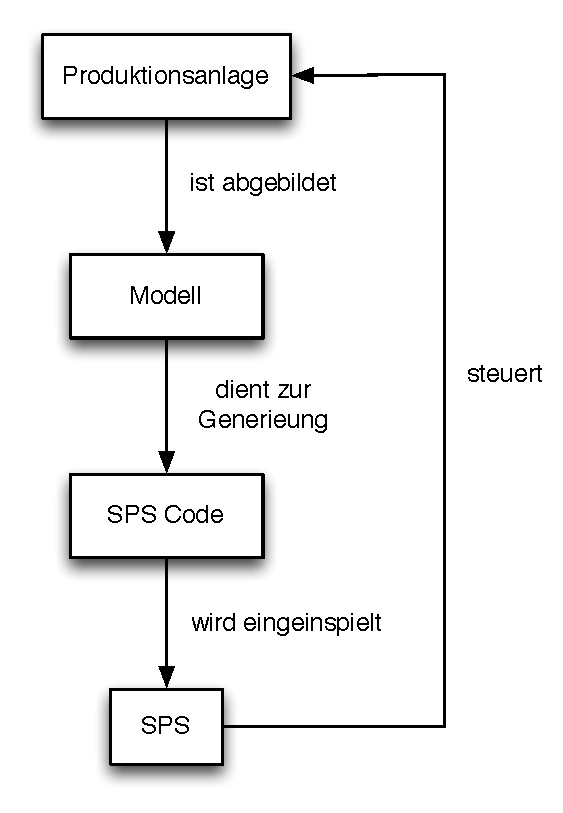
\includegraphics[width=0.37\textwidth]{graphics/konzept/konzept_allblack.pdf}
		\caption{Konzept für die modellbasierte Entwicklung der Steuerung}
		%\label{fig:MegaProxyProblem}
\end{figure} \\
Es beginnt mit einer Produktionsanlage, wobei es sich um eine Chargenprozessanlage handelt, die in einem Modell abgebildet wird. Dieses Modell beinhaltet die nötigen Daten, die gebraucht werden, um im weiteren Schritt den Code für die SPS zu generieren. Dieser Code ist nach dem IEC 61512 Standard genormt. Nachdem der Code in die SPS eingespielt wird, kann die Chargenprozessanlage gesteuert werden. 
In diesem Kapitel wird jeder Schritt, der in dem Kreislauf von Abbildung 3.1 enthalten ist, genauer elaboriert und in Perspektive zu dem entwickelten Konzept gebracht.
\section{Produktionsanlage}
\section{Modell}
Die Informationen für die Codegenerierung benötigen einerseits einen Ontologie, zur Speicherung der Informationen der Produktionsanlagen,  und andererseits ein Aktivitätsdiagramm. In diesem werden die Wege (Phasen) dargestellt, die später möglich sein sollen.
Die beiden sind von einander Abhängig, denn die Namen, der von in der Ontologie erstellen Identitäten (Datensätze), werden den Namen des Aktivitätsdiagramms zugeordnet.
Mithilfe der Ontologie und des Aktivitätsdiagramms können die Informationen bereitgestellt werden, die für die Codegenerierung nötige sind.  

\subsection{Abbildung der Produktionsanlage}
Hierbei handelt es sich um die Speicherung der Daten der Produktionsanlage in einer Ontologie. Zu den Daten gehören folgende Informationen. 
Die Abbildung der Produktionsanlage  

\subsection{Abbildung der Wege}
Bei der Abbildung der Wege wird die 
Die Abbildung der Wege werden mit eine Activity Diagram nach der UML Norm erstellt.
\begin{figure}[h!]
		\centering
		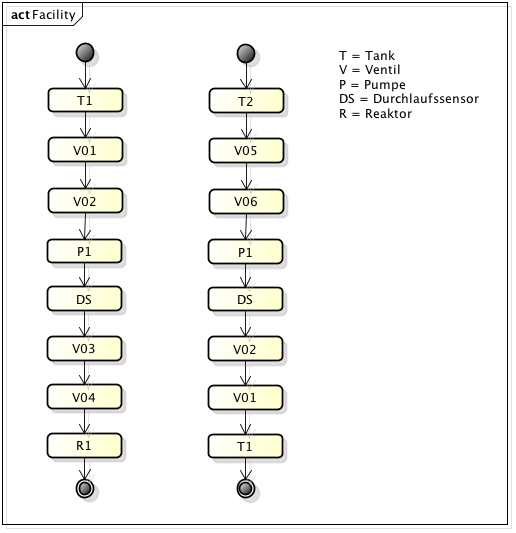
\includegraphics[width=0.8\textwidth]{graphics/konzept/UML_Activity.png}
		\caption{Abbildung der Wege mittels Activity Diagram}
		%\label{fig:MegaProxyProblem}
\end{figure}

\section{SPS Code}
\subsection{Phasen}
\subsection{Rezepte}
\section{Codegenerierung}
\section{Visualisierung der Produktionsanlage}

